\documentclass{beamer}

\usetheme{CambridgeUS}

\title[Wideband Fading Models]{Wideband Fading Models Summary}
\author{Alireza Mousazadeh \\
	mousazadealireza8@gmail.com}
\date{\today}

\begin{document}

\begin{frame}
	\titlepage
\end{frame}

%------------------------------------------

\begin{frame}{Narrowband vs. Wideband Channels}
	
	Gist of the topic
	\begin{itemize}
		\item \textbf{Narrowband:}
		\begin{itemize}
			\item Bandwidth small relative to delay spread
			\item Multipath overlaps → flat fading, minimal ISI(\textit{intersymbol interference})
		\end{itemize}
		\item \textbf{Wideband:}
		\begin{itemize}
			\item Bandwidth large enough to resolve multipath
			\item Causes frequency-selective fading and ISI
		\end{itemize}
	\end{itemize}
\end{frame}

\begin{frame}
	\begin{figure}
		\centering
		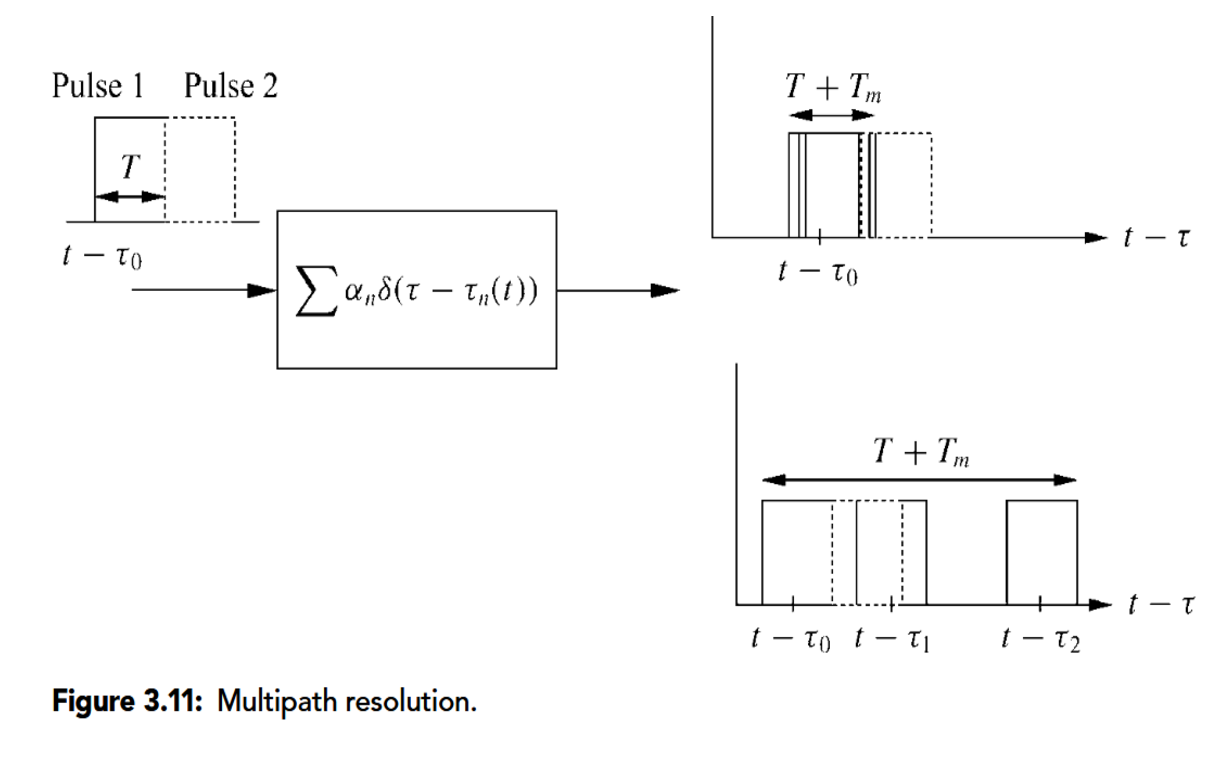
\includegraphics[width= \linewidth]{./img/3-11.eps}
	\end{figure}
\end{frame}
%------------------------------------------

\begin{frame}{Time-Varying Channel Model}
	\begin{itemize}
		\item Channel represented by impulse response \( c(\tau, t) \)
		\begin{itemize}
			\item \( \tau \): multipath delay
			\item \( t \): channel time variation
		\end{itemize}
		\item Scattering function \( S_c(\tau, \rho) \)
		\begin{itemize}
			\item \(S_c(\tau, \rho)\) is fourier transform of impulse response with respect to \(t\) called \textit{deterministic scattering function}
			\item Describes multipath energy over delay and Doppler
		\end{itemize}
	\end{itemize}
\end{frame}

%------------------------------------------

\begin{frame}{WSSUS Channel Model}
	\begin{itemize}
		\item \textbf{Wide-Sense Stationary (WSS)}:
		\begin{itemize}
			\item Statistics depend only on time difference
			\item \(E[c(\tau, t)]\) is constant
			\item \(A_{c}(t_1, t_2)\) is only a function of \(t_1 - t_2\)
		\end{itemize}
		\item \textbf{Uncorrelated Scattering (US)}:
		\begin{itemize}
			\item Multipath components with different delays are uncorrelated
		\end{itemize}
		\item Enables simplified channel analysis:
		\begin{itemize}
			\item Power delay profile
			\item Autocorrelation functions
			\item Scattering function
		\end{itemize}
	\end{itemize}
\end{frame}

%------------------------------------------

\begin{frame}{Power Delay Profile \& Delay Spread}
	\begin{itemize}
		\item Power delay profile \( A_c(\tau) \): average power vs. delay
		\item it can be shown that \(S_c(\tau, \rho) = \int A_c(\tau,\Delta t) e^{(-j2\pi\rho\Delta t)}d\Delta t\)	
		\item Metrics:
		\begin{itemize}
			\item Mean delay spread \( \mu_{T_m} \)
			\item RMS delay spread \( \sigma_{T_m} \)
		\end{itemize}
		\item ISI becomes significant when:
		\[
		T_s \lesssim \sigma_{T_m}
		\]
	\end{itemize}
	\begin{figure}[bht]
	\centering
	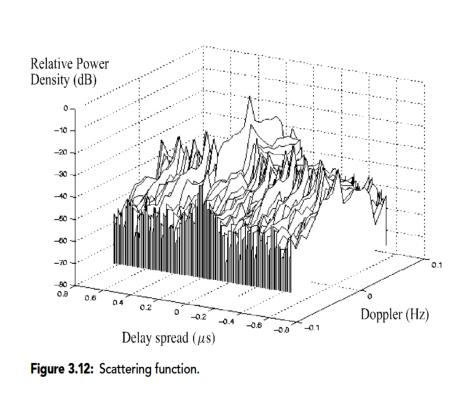
\includegraphics[scale=.5]{./img/3-12.eps}
	\end{figure}
\end{frame}

%------------------------------------------

\begin{frame}{Coherence Bandwidth}
	\begin{itemize}
		\item Coherence bandwidth:
		\begin{figure}[tbh]
		\centering
		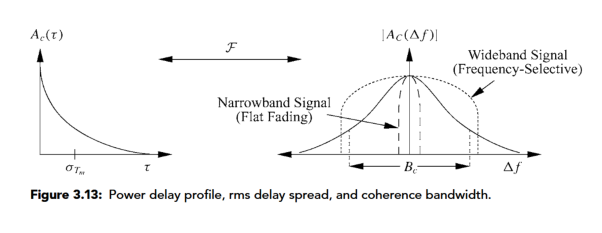
\includegraphics[scale=.6]{./img/3-13.eps}
		\end{figure}
		\item \(A_C(\Delta f) = \int A_c(\tau)e^{-j2\pi \Delta f \tau}d\tau\)
		\[
		B_c \approx \frac{1}{\sigma_{T_m}}
		\]
		\item Describes frequency range with correlated fading
		\item If signal bandwidth:
		\begin{itemize}
			\item \( B \ll B_c \) → flat fading
			\item \( B \gg B_c \) → frequency-selective fading
		\end{itemize}
	\end{itemize}

\end{frame}

%------------------------------------------

\begin{frame}{Doppler Spread \& Coherence Time}
	\begin{itemize}
		\item Caused by motion of transmitter/receiver
		\item Doppler spread \( B_D \): max Doppler shift
		\item Coherence time:
		\[
		T_c \approx \frac{1}{B_D}
		\]
		\item Higher speed → larger Doppler → smaller coherence time
	\end{itemize}
		\begin{figure}[hbt]
		\centering
		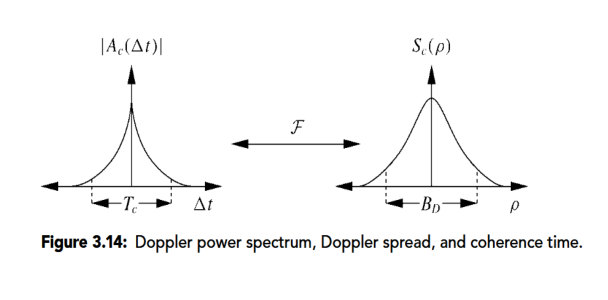
\includegraphics[scale=.6]{./img/3-14.eps}
	\end{figure}
	
\end{frame}

%------------------------------------------

\begin{frame}{Transform Relationships}
	\begin{itemize}
		\item Delay–frequency duality via Fourier transforms
		\item Time correlation ⇄ Doppler spectrum
		\item Scattering function links:
		\begin{itemize}
			\item Delay profile
			\item Doppler spectrum
			\item Frequency correlation
			\item Time correlation
		\end{itemize}
		
	\end{itemize}
	\begin{figure}[hbt]
		\centering
		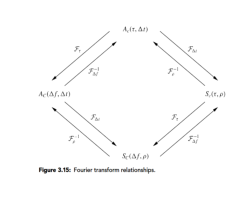
\includegraphics[scale=1.4]{./img/3-15.eps}
	\end{figure}
\end{frame}


\end{document}
